% --------------------------------------------------------------------------- %
\chapter{Measurement and Data Processing}
\label{chap:measurementProcess}
% --------------------------------------------------------------------------- %

\todo[inline]{%
    Primary questions to answer in this chapter: What did we measure, how, and
    why?
}

The goal in this project was to  create an efficient, streamlined workflow for
measuring multiple sensor chips  and  correlating  the  results  in meaningful
ways.  The  conclusions  drawn  in  this  report  mostly  originated  from  DC
measurements;  A  number of known voltages are applied to the chip's input and
its output is observed. There are multiple  configurations  to  do  this with,
namely  in  function of the preamp gain and the sampling frequency $fs$, which
in  turn  can  be  done  again as a whole for just the preamp,  for  just  the
$\Sigma\Delta$C or for both combined (the whole chip). These measurements were
performed on 10 different chips that all originated from the same wafer.  This
gives us some statistical reinforcement in  the  results,  assuming  the whole
wafer isn't biased of course.

\begin{figure}[t]
    \centering
    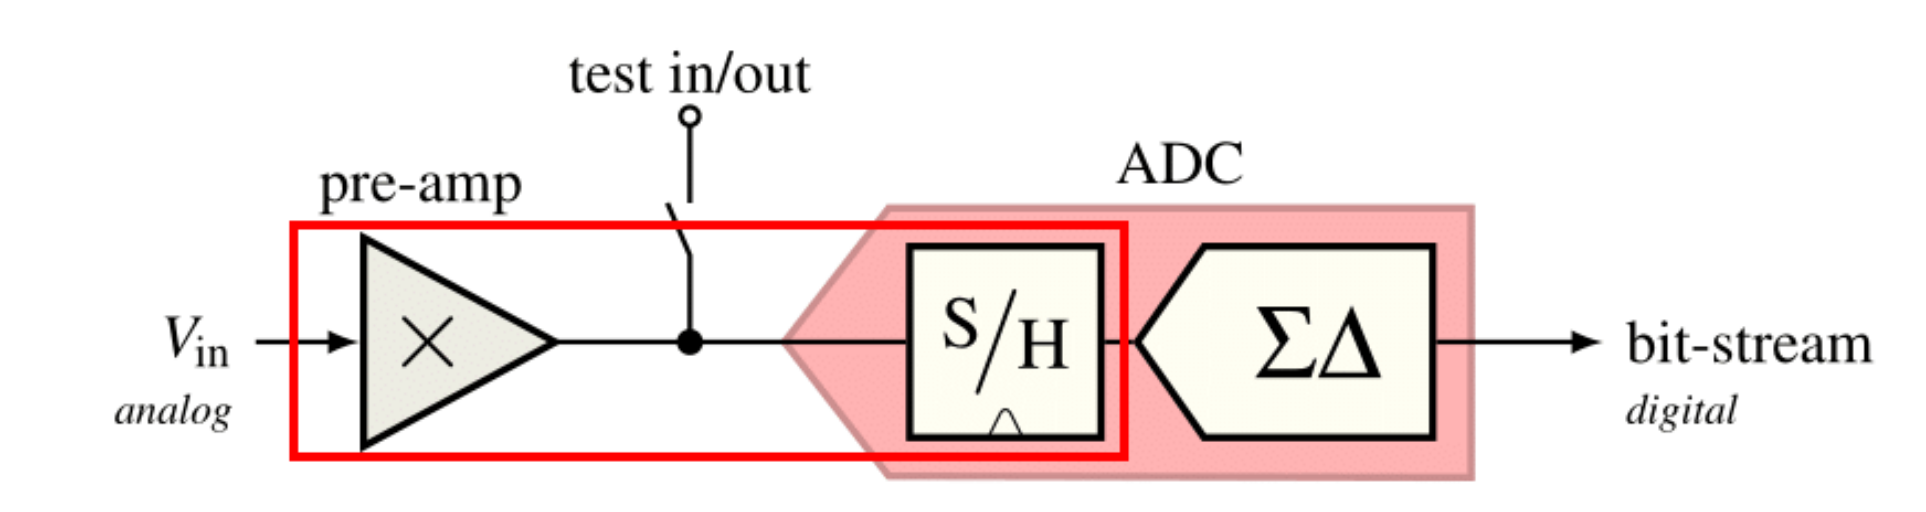
\includegraphics[width=.8\linewidth]{images/blockdiagram.png}
    \caption{Rough block diagram of the sensor chip}
    \label{fig:blockdiagram}
\end{figure}

Figure \ref{fig:blockdiagram} shows a rough overview of the chip's components.

The preamp is responsible for amplifying the difference of an input voltage to
a  $\SI{1.5}{\volt}$ reference voltage by an  externally  configurable  factor
(either  by  1,  2,  4,  8,  or 16). Additionally, the amplifier can be set to
invert the gain.

The   SAH   (Sample   and    Hold)    block    works    together    with   the
$\Sigma\Delta$-Modulator  to convert the analog voltage from the preamp into a
digital bit-stream.

There are two different  kinds  of measurements which had to be performed: The
output from measurements involving the \sdm were recorded using  a GPIO pin on
a  \raspi.  Here,  the  input  signal  is  either  applied to the preamp (when
measuring the whole  device)  or  to the \signal{TEST OUT} pin (when measuring
the \sdm alone). The output from the preamp on the other hand is analog, so it
needed to  be  measured  using  an oscilloscope via the \signal{TEST OUT} pin.

For both the preamp as well as the \sdm, DC measurements over an input voltage
range   between   \SI{0.5}{\volt}  and  \SI{2.5}{\volt}  were  performed.   AC
measurements  are  used   to   assess   the   system's   frequency   behavior.

The sample size is 10 chips, unless indicated otherwise.

Based on these  measurements and their analysis in the next chapter, we strive
to answer the question of what sort of use cases this system  is suitable for,
and with which settings.

% TODO: noise
% TODO: resolution in bits under a given set of circumstances
% TODO: Measurement methodology


% --------------------------------------------------------------------------- %
\section{Pre-Amplifier: DC Measurements}
\label{sec:preAmpDC}
% --------------------------------------------------------------------------- %



% --------------------------------------------------------------------------- %
\section{Sigma-Delta Converter: DC Measurements}
\label{sec:sigdelDC}
% --------------------------------------------------------------------------- %

% --------------------------------------------------------------------------- %
\section{Complete System: DC Measurements}
\label{sec:systemDC}
% --------------------------------------------------------------------------- %

